This section walks through the algorithm step by step, so as to explain
which
methods are used and how they are implemented.
The idea is that the code from step \mcode{S01_..} on can only accept one well
defined structure of data. In earlier versions the approach was to write code
that would adapt to different types of data automatically. All of this extra
adaptivity turned out to visually and structurally clog the code more than it
did offer much of a benefit. The concept was therefor reversed.
\mcode{S00_prep_data} can be altered to produce required output. Yet, there
should be no need to adapt any of the later steps in any way.
All input parameters are to be set in \mcode{input_vars.m}.
%%%%%%%%%%%%%%%%%%%%%%%%%%%%%%%%%%%%%%%%%%%%%%%%%%%%%%%%%%%%%%%%%%%%%%%%%%%%%%%%
%%%%%%%%%%%%%%%%%%%%%%%%%%%%%%%%%%%%%%%%%%%%%%%%%%%%%%%%%%%%%%%%%%%%%%%%%%%%%%%%
\section{Step S00: Prepare Data}
\mcode{function S00_prep_data}	\\
Before the actual eddy detection and tracking is performed,  SSH-, latitude- and longitude-data is extracted from the given data at desired geo-coordinate bounds and saved as structures in the form needed by the next step (S01).
\subsection{S00: Set Up}
\mcode{function [DD]=set_up}\\
The main purpose of this step is to Find the boundary-indices in the data
describing a window that includes the user-chosen geo-coordinate window. 
\subsection{S00: Parallel Part}
\mcode{function spmd_body(DD)}\\
This function distributes chunks of data (\ie bins of files) to the threads, which then perform the cutting and save their outputs to \mcode{'../DATA/CUTS/'}.
 The code can handle geo-coordinate input that crosses the longitudinal seam of
the input data. \Eg say the input data comes in matrices that start and end on
some (not necessarily strictly meridional) line straight across the Pacific and
it is the Pacific only that is to be analyzed for eddies, the output maps are
stitched accordingly. If the desired range is zonally continuous \eg the entire
southern ocean, the first tenth (zonally) of the input data is appended to the
end of the output. This ensures that eddies right on the seam can be found and
that eddies can be tracked across the seam. This results in eddies being
identified twice in \mcode{function S03_filter_eddies.m} \todo{ref}. Such
\textit{phantom} eddies are filtered out in \mcode{S04_track_eddies}.

%%%%%%%%%%%%%%%%%%%%%%%%%%%%%%%%%%%%%%%%%%%%%%%%%%%%%%%%%%%%%%%%%%%%%%%%%%%%%%%%
%%%%%%%%%%%%%%%%%%%%%%%%%%%%%%%%%%%%%%%%%%%%%%%%%%%%%%%%%%%%%%%%%%%%%%%%%%%%%%%%

 \section{Step S01: Find Contours}
\mcode{function S01_contours}\\
The sole purpose of this step is to apply MATLAB's \mcode{contourc.m} function
to the SSH data. It simply saves one file per time-step with all contour indices
appended into one vector \footnote{see the MATLAB documentation.}. The contour
intervals are determined by the user defined increment and range from the
minimum- to the maximum of given SSH data. \\
The function \mcode{initialise.m}, which is called at the very beginning of
every step, here has the purpose of rechecking the \textit{cuts} for
consistency and correcting the time-steps accordingly (\ie when files are
missing). \mcode{initialise.m} also distributes the files to the threads \ie
parallelization is in time dimension.
\section{Step S01b: Find Mean Rossby Radii and Phase Speeds}
\mcode{function S01b_BruntVaisRossby}\\
\todo{TODO!}


\section{Step S02: Calculate Geostrophic Parameters}
\mcode{function S02_infer_fields}\\ 
This step reads the cut SSH data from \mcode{S00_prep_data} to
\begin{itemize}
	\item  use one of the files' geo-information to determine $\f$, $\dfdy$,
$\g$ and the ratio $\g/\f$.
\item
 calculate geostrophic fields from SSH gradients.
 \item
 calculate deformation fields (vorticity, divergence, stretch and shear) via the
fields supplied by the last step.
\item calculate $\okubo$.
\end{itemize}

%%%%%%%%%%%%%%%%%%%%%%%%%%%%%%%%%%%%%%%%%%%%%%%%%%%%%%%%%%%%%%%%%%%%%%%%%%%%%%%%
%%%%%%%%%%%%%%%%%%%%%%%%%%%%%%%%%%%%%%%%%%%%%%%%%%%%%%%%%%%%%%%%%%%%%%%%%%%%%%%%

\section{Step S03: Filter Eddies}
\mcode{function S03_filter_eddies}\\ 
Since indices of all possible contour lines at chosen levels are available at
this point, it is now time to subject each and every contour to a
myriad of tests to decide whether it qualifies as the outline of an eddy as
defined by the user input threshold parameters.
\subsection{Reshape for Filtering}
\mcode{function eddies2struct}\\
In the first step the potential eddies are transformed to a more sensible
format, that is, a structure \mcode{Eddies(EddyCount)} where \mcode{EddyCount}
is the number of all contours. The struct has fields for level, number of
vertices, exact \ie interpolated coordinates and rounded integer coordinates.
\subsection{Correct out of Bounds Values}
\mcode{function CleanEddies}\\
The interpolation of \mcode{contourc.m} sometimes creates indices that are
either smaller than $0.5$ or larger than $N+0.5$ \footnote{where $N$ as the
domain size} for contours that lie along a boundary. After rounding, this
seldomly leads to indices of either $0$ or $N+1$. These values get set to $1$
and $N$ respectively in this step.
\subsection{Descent/Ascend Water Column and Apply Checks}
The concept of this step is a direct adaption of the algorithm described
by \cite{Chelton2011}. It is split into two steps, one for anti-cyclones and one
for cyclones. Consider \eg the anti-cyclone situation. Since all
geostrophic anti-cyclones are regions of relative high pressure, all
anti-cyclones \footnote{henceforth abbreviated AC} effect an elevated \SSH \ie
a \textit{hill}. The algorithm ascends the full range SSH levels where
contours were found. Consider an approximately Gaussian shaped AC that has a
peak SSH of say 5 increments larger than the average surrounding waters. 
As the algorithm approaches the sea surface from below, it will eventually run
into contours that are closed onto themselves and that encompass the AC. At
first these contours might be very large and encompass not only one but several
ACs and likely also cyclones, but as the algorithm continues upwards found
contour will get increasingly circular, describing some outer \textit{edge} of
the AC. Once the contour and its interior pass all of the tests the algorithm
will decide that an AC was found and write it and all its parameters to disk.
The AC's region \ie the interior of the contour will be flagged from here on.
Hence any inner contour further up the water column will not pass the tests.
Once all AC's are found for a given time-step, the SSH flags get reset and the
entire procedure is repeated only this time \textit{descending} the SSH-range to
find cyclones. The tests for cyclones and anti-cyclones are identical except for
a factor $-1$ where applicable. In the following the most important steps of the
analysis are
outlined. 
\subsubsection{NaN-Check Contour}
\mcode{function CR_RimNan}\\
The first and most efficient test is to check whether indices of the
contour are already flagged. Contours within an already found eddy get thereby
rejected immediately.
\subsubsection{Closed Ring}
\mcode{function CR_ClosedRing}\\
Contours that do not close onto themselves are obviously not eligible for
further testing.
\subsubsection{Sub-Window}
\mcode{function get_window_limits}\\
\mcode{function EddyCut_init}\\
For further analysis a sub-domain around the eddy is cut out of the SSH data.
These functions determine the indices of that window and subtract the
resultant offset for the contour indices. 
\subsubsection{Logical Mask of Eddy Interiour}
\mcode{function EddyCut_mask}\\
Basically this function creates a
\href{http://en.wikipedia.org/wiki/Flood_fill}{flood-fill} logical mask of the
eddy-interior. This is by far the most calculation intensive part of the whole
filtering procedure. A lot more time was wasted on attempting to solve this
problem more efficiently than time could have been saved would said attempts
have
been successful. The current solution is basically just MATLAB's
\mcode{imfill.m}, which was also used in the very first version of 09/2013.
\subsubsection{Islands}
\mcode{function CR_Nan}\\
No flags within the eddy are allowed. This check also avoids contours around
islands as all land is flagged \textit{a priori}.
\subsubsection{Sense}
\mcode{function CR_sense}\\
\textbf{All} of the interior SSH values must lie either above or below current
contour level, depending on whether anti-cyclones or cyclones are sought.
\subsubsection{Area} \label{filter:area}
\mcode{function EddyCircumference}\\
Area described by the contour. This is needed for \ref{filter:shape}. This is
not however related to the actual eddy scale determined in
\ref{filter:dynscale}.
\subsubsection{Cirumference}
\mcode{function EddyCircumference}\\
Line-length (sum of Euclidean norm of all nodes) of the contour.
\newpage
\subsubsection{Shape}\label{filter:shape}
\mcode{function CR_Shape}\\
\begin{wrapfigure}{r}{0.4\textwidth}
	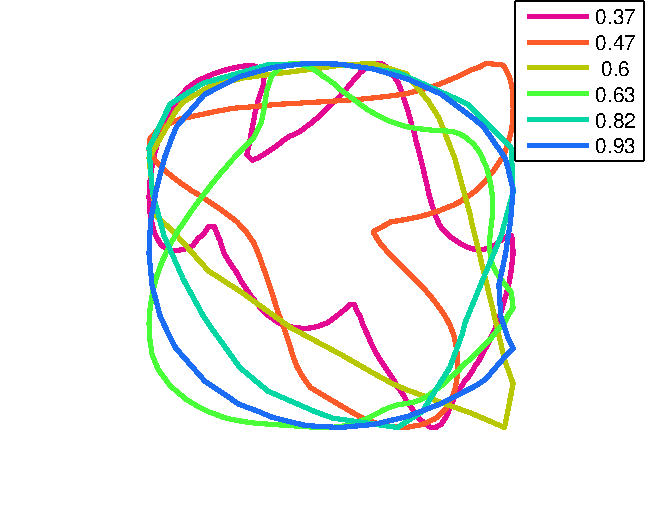
\includegraphics[width=0.45\textwidth]{isoper}
	\caption{Different values of the isoperimetric quotient.}
	\label{fig:isoper}
\end{wrapfigure}

This is the crucial part of deciding whether the object is \textit{round
enough}. A perfect vortex with $\dpr{u}{y}=-\dpr{v}{x}$ is necessarily a
circle. The problem is that eddies get formed, die, merge, run into obstacles,
get asymmetrically advected etc. To successfully track them it is therefor
necessary to allow less circle-like shapes whilst still avoiding to \eg count 2
semi merged eddies as one. 
This is achieved by calculating the \hyperref[def:IQ]{isoperimetric quotient},
defined as the ratio of a ring's area to the area of a circle with equal
circumference. \cite{Chelton2011} use a similar method. They
require:\\ \textit{The distance between any pair of points within the connected
region must be less than a specified maximum} \citep{Chelton2011}.\\
While this method clearly avoids overly elongated shapes it allows for stronger
deformation within its distance bounds. \todo{compare both, show pictures}
\subsubsection{Amplitude} \label{filter:amp}
\mcode{function CR_AmpPeak}\\
This function determines the amplitude \ie the maximum of the absolute
difference between SSH and current contour level and the position thereof as
well as the amplitude relative to the mean SSH value of the eddy interior as
done by \cite{Chelton2011}. The
amplitude is then tested against the user-given threshold. The function also
creates a matrix with current contour level shifted to zero and all values
outside of the eddy set to zero as well. 
\subsubsection{Profiles}
\mcode{function EddyProfiles}\\
This step saves the meridional and zonal profiles of SSH, U and V. 
\begin{wrapfigure}{r}{0.4\textwidth}
	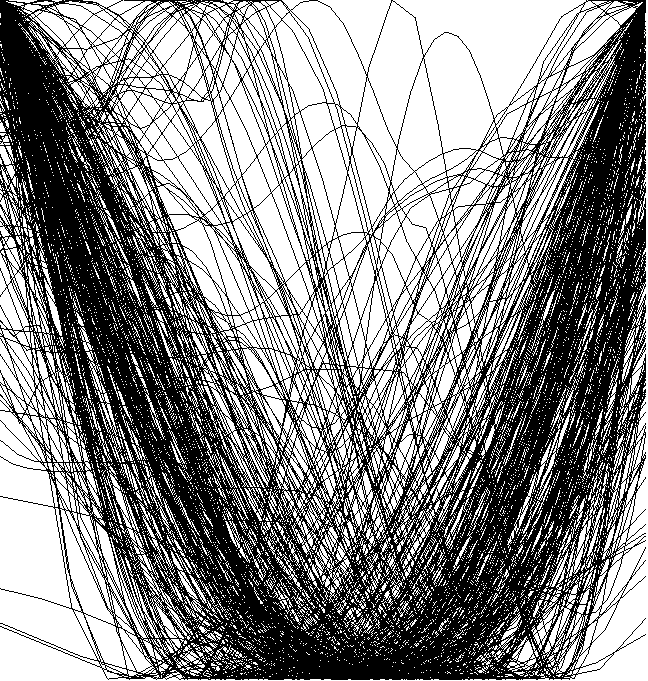
\includegraphics[width=0.4\textwidth]{profiles}
	\caption{Zonal $x$- and $z$-normalized cyclone-profiles.}
	\label{fig:profiles}
\end{wrapfigure}

\subsubsection{\textit{Dynamic} Scale} \label{filter:dynscale}
\mcode{function EddyRadiusFromUV}\\
The contour line that is being used to detect the eddy is not
necessarily a good measure of the eddy's \textit{scale} \ie it doesn't
necessarily represent the eddy's outline very well. This becomes very 
obvious when the area, as inferred by \ref{filter:area}, is plotted over time
for an already successfully tracked eddy. The result is not a smooth curve at
all. This is so because at different time steps the eddy usually gets detected
at different contour levels. Since its surrounding continuously changes and
since the eddy complies with the testing-criteria the better the closer the
algorithm gets to the eddy's peak value, the determined area of the contour
jumps considerably between time steps. This is especially so for large flat
eddies with amplitudes on the order of $1cm$. If the contour increment is on
that scale as well, the difference in contour-area between two time steps 
easily surpasses $100\%$ and more. 
Since there is no definition for the \textit{edge} of an eddy, it is here
defined as the ellipse resulting from the meridional and zonal diameters that
are the distances between first minimum and maximum orbital velocity, away from
the eddy's peak in positive and negative y and x directions respectively. 
In the case of a meandering jet with a maximum flow speed at its center, that
is shedding off an eddy, this scale corresponds to half the distance between
two opposing center-points of the meander. It is also the distance at which a
change in vorticity polarity occurs and is thus assumed to be the most plausible
\textit{dividing line} between vortices. 
\todo{theres probably a better way via okubo weiss!}
In practice the velocity-gradient profiles need to be smoothed to successfully
determine their first adequate zero-crossing. Once the zero crossings in all
4 directions are found, their mean is taken as the eddy's scale. Note that this
is again similar to what \cite{Chelton2011} did. 
\subsubsection{\textit{Dynamic} Amplitude}
\mcode{function EddyAmp2Ellipse}\\
As mentioned above, the contour that helps to detect the eddy is not
representative of its extent. This is also true for the $z$-direction, for the
same reasons. This function therefor takes an SSH-mean at indices of the ellipse
created by the determined zonal and meridional \textit{dynamical} diameters,
and uses this as the basal value to determine a \textit{dynamic} amplitude.
\subsubsection{Center of Volume}
\mcode{function EddyArea2Ellipse}\\
\mcode{function CenterOfVolume}\\
Instead of using the geo-position of the eddy's peak in the tracking procedure,
it was decided to instead use the center of the volume created by the basal
shifted matrix from \ref{filter:amp} \ie \textit{the center of volume of the
dome
(resp. valley) created by capping off the eddy at the contour level}.
This method was chosen because from looking at animations of the tracking
procedure
it became apparent that, still using peaks as reference points, the eddy
sometimes jumped considerably from one time step to the next if two local maxima
existed within the eddy. \Eg in one time-step local maximum $A$ might be just a
little bit larger than local maximum $B$ and one time-step later a slight shift
of mass pushes local maximum $B$ in pole position, creating a substantial jump
in the eddy-identifying geo-position hence complicating the tracking procedure. 
\section{Step S04: Track Eddies}
\mcode{function function S04_track_eddies}\\
Due to the the relatively fine temporal resolution (daily) of the model data,
the tracking procedure turns out to be much simpler than the one described by
\cite{Chelton2007}. There is really no need to project the new position of an
eddy, as it generally does not travel further than its own scale in one day.
This means that one eddy can be unambigiously tracked from one time step to the
next as long both time-steps agree on which eddy from the other
time-step is located the least distance away.
The algorithm therefor simply builds an arc-length-distance matrix
between all old and all new eddies and then determines the minima of that
matrix in both directions \ie one array for the new with respect to the old,
and one for the old with respect to the new set. This leads to the following
possible situations:
\begin{itemize}
	\item 
	Old and new agree on a pair. \Ie old eddy $O_a$ has a closest neighbour in
the new set $N_a$ and $N_a$ agrees that $O_a$ is the closest eddy from the old
set. Hence the eddy is tracked.  $N_a$ is $O_a$ at a later time.
\item
$N_a$ claims $O_a$ to be the closest, but $N_b$ makes the same claim. \Ie two
eddies from the new set claim one eddy from the old set to be the closest. 
In this situation the closer one is decided to be the old one at a later
time-step and the other one must be a newly formed eddy.
\item 
At this point all new eddies are either allocated to their respective old
eddies or assumed to be \textit{newly born}. The only eddies that have not been
taken care of are those from the old set, that \textit{lost} ambigious claims to
another old eddy, that was closer to the same claimed new eddy. \Ie there is no
respective new eddy available which must mean that the eddy just \textit{died}.
In this case the entire track with all the information for each time step is
saved as long as the track-length meets the threshold criterium. If it doesn't,
the track is deleted. 
\end{itemize}

\section{Step S05: Cross Reference Old to New Indices}
\mcode{function function S05_init_output_maps}\\
The main purpose of this step is to allocate all grid nodes of the input data
to the correct node of the output map. Since the output map is usually much
coarser than the input data there is no need for interpolation.  

\section{Step S06: Make Maps of Mean Parameters}
\mcode{function function S06_analyze_tracks}\\
 

\section{Example}
To show a hands-on example an exemplary run for part of the North Atlantic is
demonstrated in the following. 
\subsection{Map Parameters} \label{codeEx:map_params}
The geo-coordinates for the map window are to be set in \mcode{map_vars.m}.
In this case a small region in the eddy-rich North Atlnatic from $-90^\circ$
west till $-40^\circ$ west and from $20^\circ$ north till $60^\circ$ north is
chosen. This script has an effect only on the very first step (\mcode{S_00..}).
\begin{lstlisting}
function MAP=map_vars
	%% user input
	MAP.geo.west=-90;
	MAP.geo.east=-40;
	MAP.geo.south=20;
	MAP.geo.north=60;
	MAP.time.delta_t = 1; % [days]
	MAP.SSH_unitFactor = 100; % eg 100 if SSH data in cm, 1/10 if in deka m etc..
	MAP.pattern.in='SSH_GLB_t.t0.1_42l_CORE.yyyymmdd.nc';
end
\end{lstlisting}
\todo{show map}
\subsection{Other Parameters}
All other parameters are to be set in \mcode{input_vars.m}. 
\begin{itemize}
	\item 
	The maximum number of \textit{local workers} (threads) is at default settings
usually limited to 12 by Matlab. Hence 
 \begin{lstlisting}
 	U.threads.num=12;
 \end{lstlisting}
 \item 
 The data available at this point in time spans from 1994/04/02 till 2006/12/31.
Hence
 \begin{lstlisting}
 	U.time.from.str='19940402';
  	U.time.till.str='20061231';
 \end{lstlisting}
\item 
Data is available per day. Therefor \mcode{U.time.delta_t=1; } is set
to 1. This could also be changed to another value, if the user wished to skip
time-steps.
	\item \label{codeEx:data}
	The path \mcode{U.path.root='../dataXMPL/';} can be set arbitrarily. If it
does not yet exist, it will be created. It is suggested to not reuse a path,
as this could lead to inconsitencies in the data.
\item
\todo{ \mcode{	U.path.TempSalt.name='TempSalt/';}}
\item
\mcode{U.path.raw.name='/scratch/uni/ifmto/u241194/DAILY/EULERIAN/SSH/';}\\
This is where the SSH data is stored.
\item
\begin{lstlisting}
	U.contour.step=0.01; % [SI]
	U.thresh.radius=5e3; % [SI]
	U.thresh.amp=0.02; % [SI]
	U.thresh.shape.iq=0.5; % isoperimetric quotient
	U.thresh.shape.chelt=0.5; % (diameter of circle with equal area)/(maximum
distance between nodes) (if ~switch.IQ) 
	U.thresh.corners=6; % min number of data points for the perimeter of an eddy
	U.thresh.dist=1*24*60^2; % max distance travelled per day
	U.thresh.life=20; % min num of living days for saving
\end{lstlisting}
In this segment the following values are set (all in SI-units, except for
time dimension).:
	\begin{itemize}
		\item 
		The contour intervall with which to look for SSH-contours from maximum to
	minimum SSH-value.
	\item
	The minimum radius threshold for an eddy.
	\item
	The minimum amplitude threshold.
	\item
	Either the minimum $\IQ$ value or the minimum ratio of the diameter of a
circle	 with equal area over the maximum distance between nodes, depending on
which	 method is chosen (see ). 
	\item
	The minimum number of grid nodes making up the contour.
	\item
	The maximum distance-travelled-per-timestep threshold.
	\item
	The minium track-length (in time) threshold for a track to be saved.
	\end{itemize}
\item

\begin{lstlisting}
	U.dim.X=40*3+1;
	U.dim.Y=40*3+1;
	U.dim.west=-90;
	U.dim.east=-50;
	U.dim.south=20;
	U.dim.north=60;
	U.dim.NumOfDecimals=1;
\end{lstlisting}
These paramters describe the output maps, that will be created in the very end
(\eg maps of mean values). Ideally they are set to the same limits as
those set in \ref{codeEx:map_params}. \mcode{U.dim.X}/\mcode{U.dim.Y} dictate
the size of the output maps. They can be set arbitrarilly, but the format \eg
$(east-west)*n +1; \;\; n \in \mathrm{N}$ is suggested to avoid long decimals in
the coordinate matrices.
\item
\begin{lstlisting}
	U.switchs.RossbyStuff=false;
	U.switchs.IQ=true;	
\end{lstlisting}
Choose whether step \mcode{S01b_BruntVaisRossby} is to be run (needs adequate
salt and temperature files \todo{explain}) and the type of shape-testing (
\mcode{U.switchs.IQ=true}) for $\IQ$-method.
\item
The rest are less important technical things that are only relevant if the code
itself is modulated (\eg if modules are added).
\end{itemize}

%%%%%%%%%%%%%%%%%%%%%%%%%%%%%%%%%%%%%%%%%%%%%%%%%%%%%%%%%%%%%%%%%%%%%%%%%%%%%%%%
\subsection{Running the Code}
The seperate steps can be run all at once via \mcode{Sall.m} or one by one, as
long as they are started consecutively in the order indicated by their name
( \mcode{S00..}, then \mcode{S01..} \etc). \mcode{S01b} is not necessary
though. Each step saves its own files which are then read by the next step.
All output data is saved in the user given root-path from \ref{codeEx:data}.
This concept uses quite a lot of disk space and is also quite substantially
slowed by all the reading and writing procedures. The benefits, on the other
hand, are that debugging becomes much easier. If the code fails at some step,
at least all the calculations up to that step are dealt with and do not need to
be re-run. The concept also makes it easy to extend the code by further
add-ons.

\todo{plots to follow...}



\href{https://github.com/PremKolar/MT4}{see github for progress}
















